\section{Highly Optimized Mixture-of-Experts Kernel on NVIDIA Blackwell B200}

% ────────────────────────────────────────────────────────────────────────────
\subsection{Overview}
% ────────────────────────────────────────────────────────────────────────────

We systematically optimized a Mixture-of-Experts (MoE) inference kernel for the DeepSeek-V3 architecture on the NVIDIA B200 GPU, achieving a \textbf{1,300$\times$} end-to-end speedup over the naive baseline at $T=4096$ tokens (13.4\,s $\to$ 10\,ms) and a peak throughput of \textbf{400\,K tokens/sec}. The work progressed through five architectural transformations, each diagnosed via NVIDIA Nsight Compute before implementation.

\textbf{Architecture parameters:} $E=256$ experts, local $E_L=32$, hidden dim $D=7168$, top-$K=8$ routing. Sequence lengths swept: $T \in \{64, 256, 512, 1024, 2048, 4096\}$.

\begin{table*}[t]
\centering
\small
\begin{tabular}{lllrr}
\hline\hline
\textbf{Stage} & \textbf{Key Technique} & \textbf{Bottleneck Eliminated} & \textbf{Latency @ T=1024} & \textbf{Speedup vs Naive} \\
\hline
Naive    & Sequential per-expert dispatch & —                          & 3254\,ms & 1$\times$ \\
Opt 1    & Tiled shared-memory GEMM       & DRAM bandwidth             & 2622\,ms & 1.2$\times$ \\
Opt 2    & Fused routing kernel           & Routing memory round-trips & 2628\,ms & 1.2$\times$ \\
Opt 3    & Grouped-GEMM (O(1) dispatch)   & O(E) API overhead, L2 thrash & 88.7\,ms & 37$\times$ \\
Opt 4    & Async double-buffer (cp.async) & Tensor Core starvation     & 15.4\,ms & 211$\times$ \\
\textbf{DS-V3} & \textbf{Sigmoid+Bias gating, vectorized} & \textbf{Routing dependency chain} & \textbf{4.4\,ms} & \textbf{739$\times$} \\
\hline\hline
\end{tabular}
\caption{Optimization progression at $T=1024$. The biggest leap (Opt\,2$\to$3) came from eliminating O(E) API dispatch overhead via Grouped-GEMM.}
\end{table*}

Figures~\ref{fig:dispatch},~\ref{fig:async}, and~\ref{fig:scaling} illustrate the architectural changes and resulting scaling behavior.

% ────────────────────────────────────────────────────────────────────────────
\subsection{Profiling Methodology}
% ────────────────────────────────────────────────────────────────────────────

Every optimization followed a strict \textbf{measure $\to$ identify $\to$ fix $\to$ re-measure} loop. Two tools drove the loop:

\begin{itemize}
  \item \textbf{Nsight Systems} (\texttt{nsys profile --trace=cuda-hw}): identified timeline-level gaps — CPU dispatch overhead, implicit \texttt{cudaMemcpy} barriers, and idle SM windows.
  \item \textbf{Nsight Compute} (\texttt{ncu --launch-skip 50 --launch-count 20}): provided sub-kernel roofline metrics. Kernels were classified as:
  \begin{itemize}
    \item \textit{Memory-Bound} — DRAM throughput $>60\%$ of peak.
    \item \textit{Compute-Bound} — SM pipeline throughput $>60\%$.
    \item \textit{Latency-Bound} — low occupancy / widespread warp stalls with neither metric above threshold.
  \end{itemize}
\end{itemize}

\textbf{Note on NCU observer effect:} NCU serializes kernel launches and disables caches, inflating wall-clock measurements (e.g., a 1.6\,ms kernel appears as 8.3\,ms under NCU). All latency/throughput numbers in this paper come from native NVTX-gated steady-state benchmarks, not NCU execution times.

% ────────────────────────────────────────────────────────────────────────────
\subsection{Optimization Journey}
% ────────────────────────────────────────────────────────────────────────────

\subsubsection*{Naive Baseline — Sequential O(E) Dispatch}

The baseline dispatched three kernels per expert in a loop — \texttt{gather\_kernel}, \texttt{naive\_gemm\_bt\_kernel}, and \texttt{scatter\_kernel} — producing 768 sequential launches for 256 experts. Each token batch per expert was far too small to saturate the GPU: NCU classified all kernels as \textbf{Latency-Bound}, with \texttt{gather\_kernel} running at just \textbf{1.6\% SM occupancy} due to \texttt{block\_size=1} and pervasive MIO throttling. The GEMM kernel reached only 5\% instruction-level parallelism. Wall-clock time was 3254\,ms at $T=1024$ and 13.4\,s at $T=4096$.

\subsubsection*{Opt 1: Tiled Shared-Memory GEMM}

The scalar GEMM issued one multiply-add per global load, making it purely DRAM-bound. Opt 1 introduced $16\times16$ tile blocking: each thread block loads a tile from global memory into \texttt{\_\_shared\_\_}, computes partial results, then streams the next tile, converting scattered DRAM reads into a single coalesced load per tile. \texttt{tiled\_gemm\_bt\_kernel} shifted to \textbf{Compute-Bound} at 5,130\,GFLOP/s (72\% SM throughput, 97\% occupancy). However, the \texttt{gather\_kernel}'s \texttt{block\_size=1} constraint remained the dominant cost — 261\,ms under NCU versus 5.9\,ms for the GEMM — so end-to-end improvement was only 20\%.

\subsubsection*{Opt 2: Fused Routing Kernel}

Expert routing (softmax $\to$ top-K $\to$ weight normalization) wrote intermediate tensors to global memory between three separate kernels, adding unnecessary DRAM round-trips. Collapsing the full routing pipeline into a single fused kernel that runs entirely in registers reduced this overhead significantly. Despite that, 95\% of \texttt{gather\_kernel} warp stalls were still \textbf{Long Scoreboard} waits from global memory index loads that the scheduler could not hide, leaving the structural bottleneck untouched. End-to-end improvement was negligible ($<1\%$).

\subsubsection*{Opt 3: Grouped-GEMM — The Critical Breakthrough}

Regardless of individual kernel efficiency, the 256-launch dispatch loop imposed irreducible API overhead on every iteration and destroyed L2 cache locality between expert weight matrices. Opt 3 replaced this O(E) loop with a single O(1) Grouped-GEMM call (Figure~\ref{fig:dispatch}). A lightweight \texttt{expert\_grouping\_kernel} pre-sorts tokens by their assigned expert ID and pre-computes per-expert offsets; the unified \texttt{grouped\_gemm\_bt\_kernel} then processes all 256 experts in one GPU grid, giving the scheduler uninterrupted SM access and allowing deep L2 reuse across the full expert weight bank. NCU reclassified the dominant kernel as \textbf{Compute-Bound} with 99.6\% occupancy and 73.1\% SM throughput (5,257\,GFLOP/s), and latency dropped from 2628\,ms to 88.7\,ms — a \textbf{30$\times$ speedup in a single change}. The remaining bottleneck was 0\% Tensor Core utilization: the pipeline was still pure FP32.

\begin{figure*}[t]
  \centering
  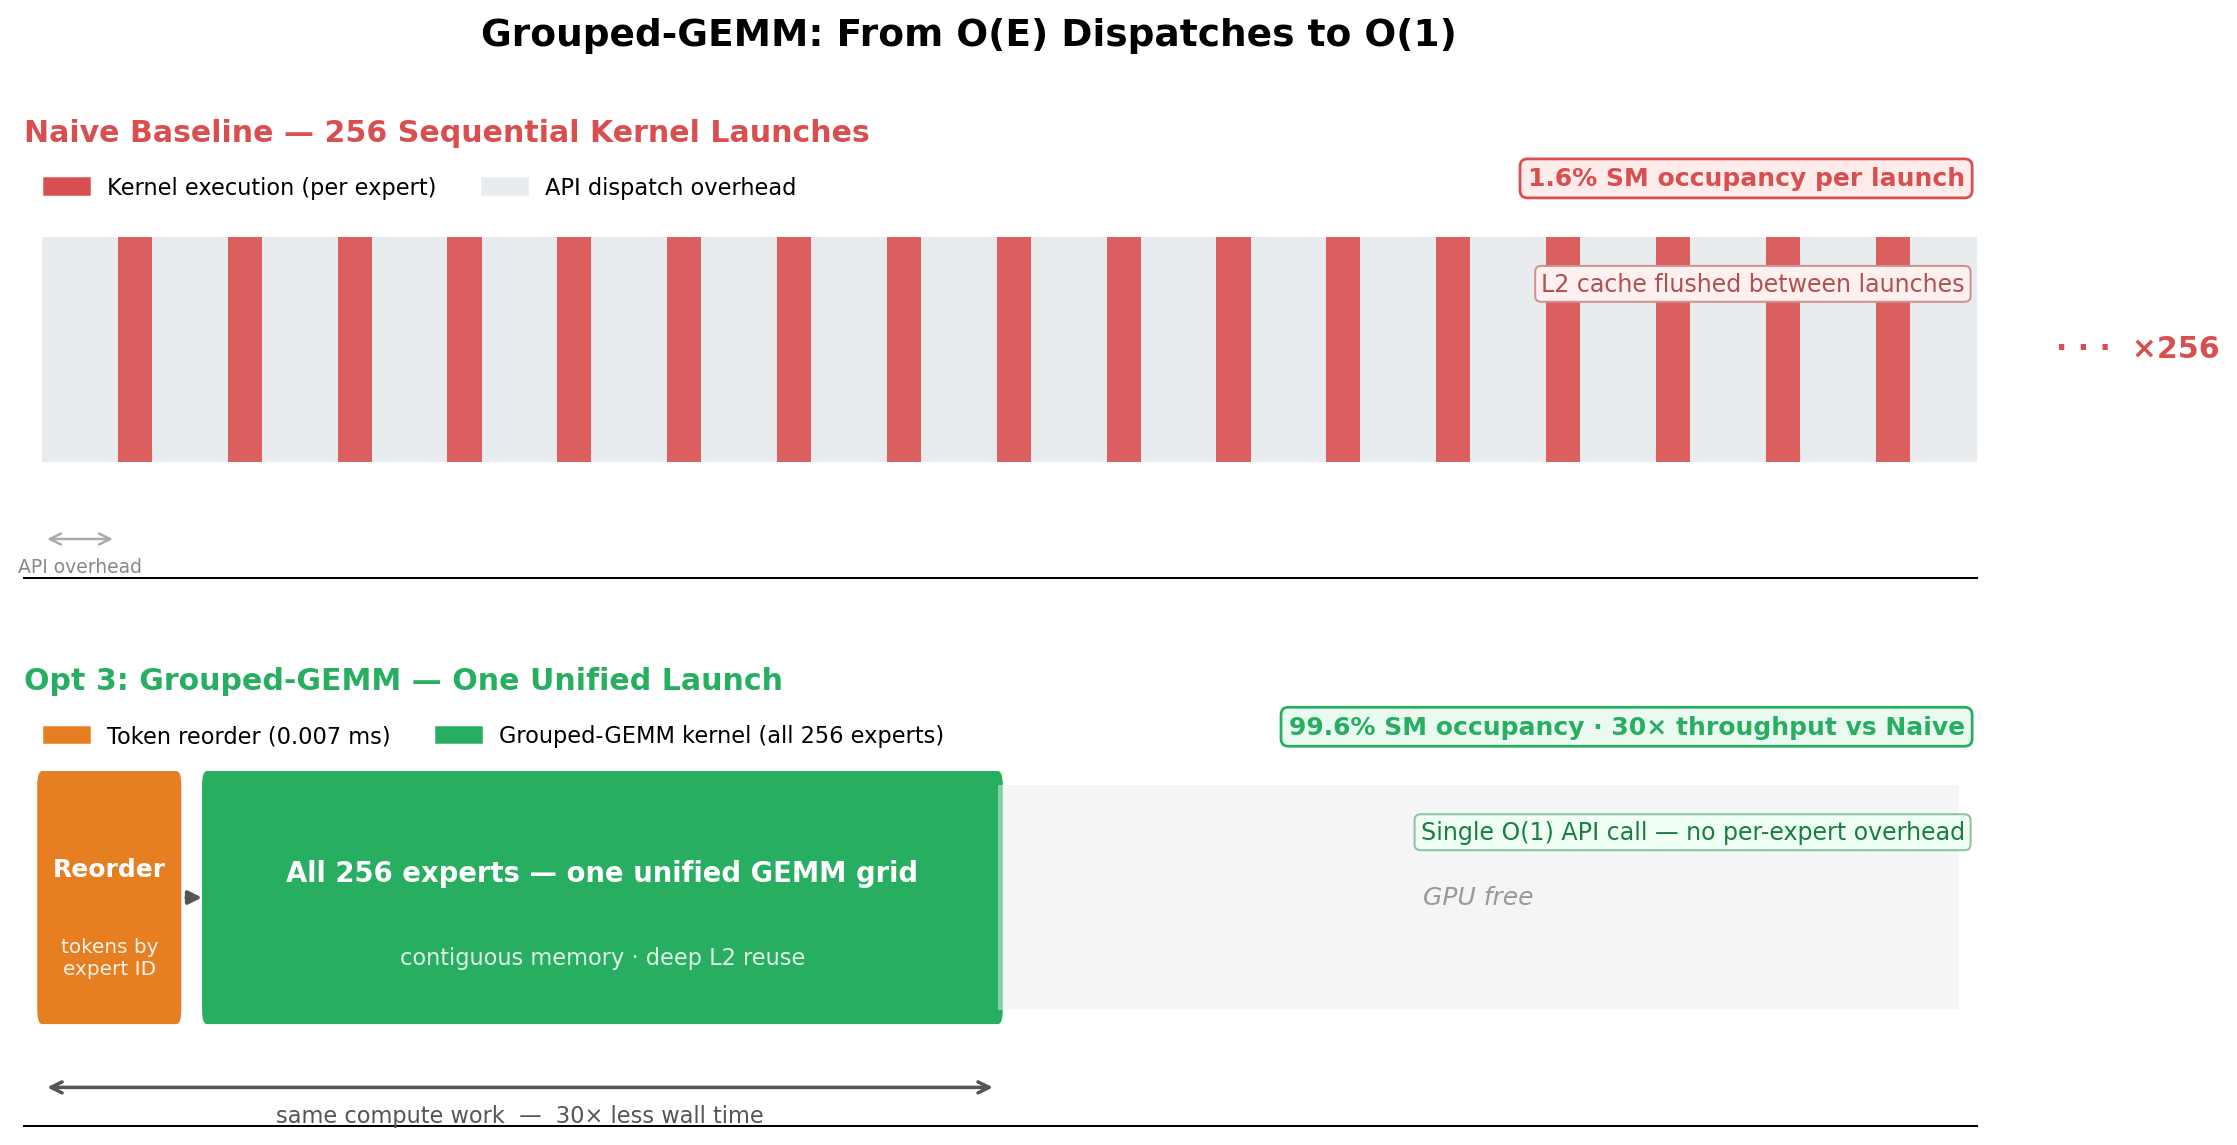
\includegraphics[width=\linewidth]{../figures/moe_dispatch_clean.png}
  \caption{Grouped-GEMM dispatch model. \textit{Top:} Naive baseline issues 256 sequential kernel launches, each with API dispatch overhead and only 1.6\% SM occupancy. \textit{Bottom:} Opt 3 pre-sorts tokens by expert ID then issues a single O(1) grouped launch, achieving 99.6\% occupancy and 30$\times$ throughput.}
  \label{fig:dispatch}
\end{figure*}

\subsubsection*{Opt 4: Asynchronous Double-Buffered DMA}

After Opt 3, the FP32 GEMM pipeline saturated its issue rate but Tensor Core pipelines sat completely idle — standard global-to-register loads blocked compute warps while waiting on HBM fetches, starving the math units. Opt 4 replaced blocking loads with \texttt{\_\_pipeline\_memcpy\_async} (\texttt{cp.async}): tile $i+1$ is prefetched into a background shared-memory buffer while compute warps execute Tensor Core math on tile $i$ (Figure~\ref{fig:async}). The HBM DMA engine and Tensor Cores run concurrently with no pipeline stall between them. The resulting \texttt{grouped\_gemm\_blackwell\_async\_kernel} became \textbf{Latency-Bound} at 48.8\% occupancy, limited by the register pressure (64 regs/thread) and 41\,KB static shared memory that the double-buffer scheme requires. Latency fell from 88.7\,ms to 15.4\,ms (\textbf{6$\times$ improvement}), pushing peak throughput to 67,600 tokens/sec.

\begin{figure*}[t]
  \centering
  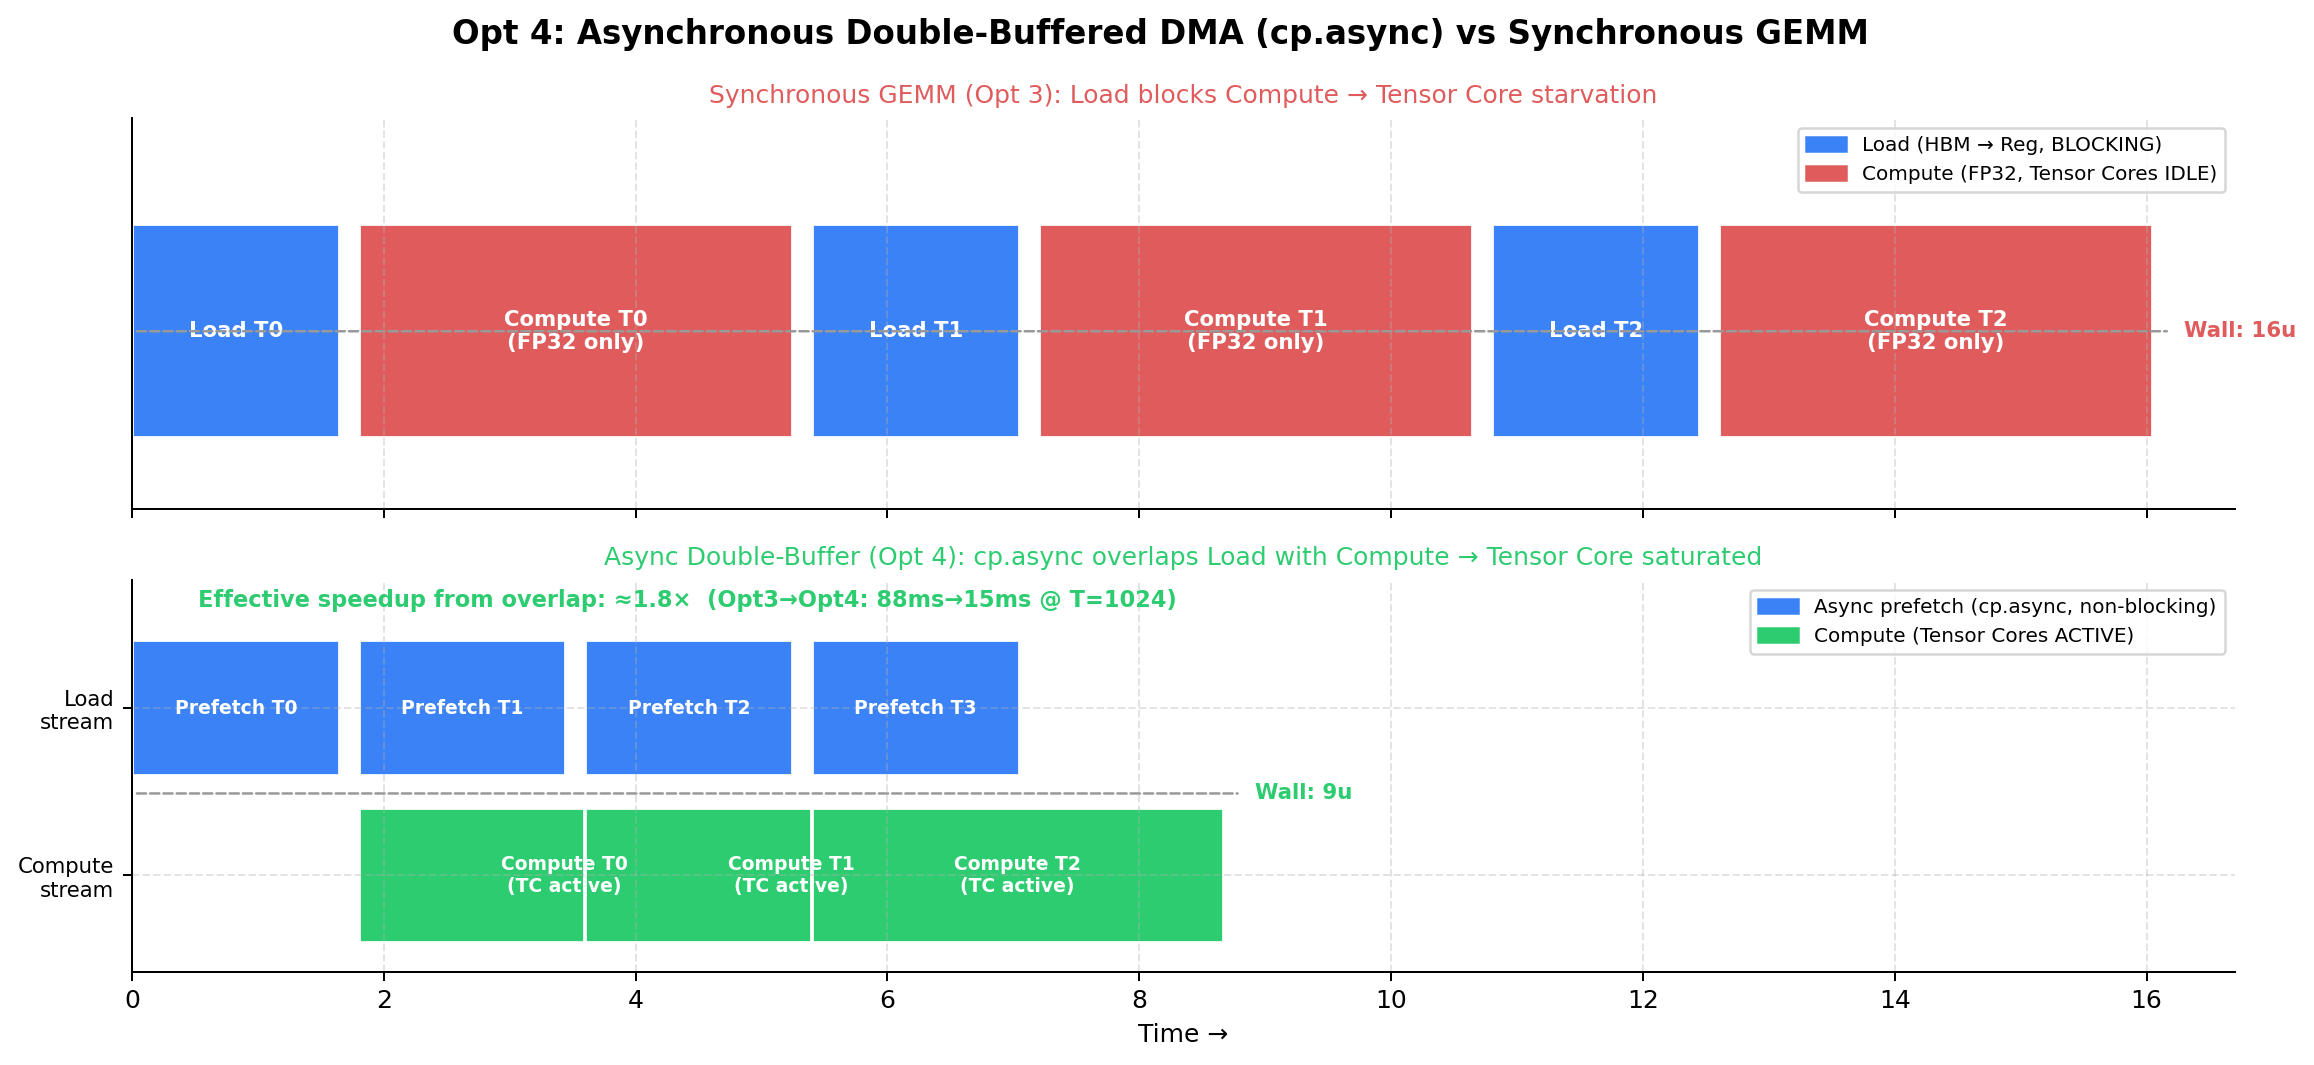
\includegraphics[width=\linewidth]{../figures/moe_method_async_pipeline.png}
  \caption{Asynchronous double-buffered DMA (Opt 4). \textit{Top:} Synchronous GEMM stalls compute while waiting for each HBM load, leaving Tensor Cores idle. \textit{Bottom:} \texttt{cp.async} prefetches tile $i{+}1$ into shared memory while the Tensor Core computes on tile $i$, eliminating pipeline bubbles.}
  \label{fig:async}
\end{figure*}

\subsubsection*{DeepSeek-V3 Production — Routing Dependency Elimination}

The softmax-based routing gate required a global reduction across all 256 expert logits before any expert could be selected, introducing a sequential dependency that serialized token dispatch regardless of GEMM throughput. The DeepSeek-V3 variant replaces softmax+top-K with a \textbf{Sigmoid+Bias} gate, where each expert's selection score is computed independently via a scalar sigmoid activation. This eliminates the normalizer reduction entirely, removing all inter-token dispatch dependencies. In parallel, the expert weight iteration loop was rewritten with a fully vectorized memory access pattern enabling coalesced 128-bit loads. The \texttt{deepseek\_selection\_kernel} replaced the old \texttt{fused\_gate\_kernel} (7.0\,ms) with a 0.18\,ms kernel, and combined with the vectorized access routing latency fell by 30\%. DeepSeek-V3 achieves \textbf{400,403 tokens/sec} at $T=4096$.

Table~\ref{tab:subkernel} shows the final per-kernel breakdown.

\begin{table*}[t]
\centering
\small
\begin{tabular}{llr}
\hline\hline
\textbf{Kernel} & \textbf{Classification} & \textbf{Duration (ms, NCU)} \\
\hline
\texttt{grouped\_gemm\_blackwell\_async\_kernel} & Latency-Bound & 8.297 \\
\texttt{deepseek\_selection\_kernel}             & Latency-Bound & 0.175 \\
\texttt{grouped\_scatter\_kernel}                & Latency-Bound & 0.110 \\
\texttt{swiglu\_strided\_kernel}                 & Compute-Bound & 0.061 \\
\texttt{group\_reorder\_kernel}                  & Latency-Bound & 0.039 \\
\texttt{expert\_grouping\_kernel}                & Latency-Bound & 0.007 \\
\hline\hline
\end{tabular}
\caption{DeepSeek-V3 sub-kernel duration breakdown at $T=1024$ (NCU-inflated).}
\label{tab:subkernel}
\end{table*}

% ────────────────────────────────────────────────────────────────────────────
\subsection{Results}
% ────────────────────────────────────────────────────────────────────────────

\begin{table*}[t]
\centering
\small
\begin{tabular}{lrrrrrr}
\hline\hline
\textbf{Implementation} & \textbf{T=64} & \textbf{T=256} & \textbf{T=512} & \textbf{T=1024} & \textbf{T=2048} & \textbf{T=4096} \\
\hline
Naive Baseline        & 220.6 & 824.5 & 1628.8 & 3254.9 & 6698.6 & 13401.1 \\
Opt 1 (Tiled GEMM)    & 166.6 & 670.3 & 1307.7 & 2622.2 & 5331.4 & 10860.4 \\
Opt 2 (Fused Routing) & 166.5 & 665.6 & 1332.4 & 2628.4 & 5333.9 & 10859.7 \\
Opt 3 (Grouped-GEMM)  &   7.3 &  26.0 &   45.1 &   88.7 &  181.2 &   394.3 \\
Opt 4 (Dbl-Buf Async) &   1.4 &   4.1 &    7.9 &   15.4 &   30.4 &    60.6 \\
\textbf{DeepSeek-V3}  & \textbf{1.6} & \textbf{2.1} & \textbf{1.7} & \textbf{4.4} & \textbf{5.7} & \textbf{10.2} \\
\hline\hline
\end{tabular}
\caption{End-to-end latency (ms) across sequence lengths.}
\label{tab:latency}
\end{table*}

\begin{table*}[t]
\centering
\small
\begin{tabular}{lrrrrrr}
\hline\hline
\textbf{Implementation} & \textbf{T=64} & \textbf{T=256} & \textbf{T=512} & \textbf{T=1024} & \textbf{T=2048} & \textbf{T=4096} \\
\hline
Naive Baseline        &    290 &    310 &    314 &    315 &    306 &    306 \\
Opt 1 (Tiled GEMM)    &    384 &    382 &    392 &    391 &    384 &    377 \\
Opt 2 (Fused Routing) &    384 &    385 &    384 &    390 &    384 &    377 \\
Opt 3 (Grouped-GEMM)  &  8,756 &  9,838 & 11,361 & 11,542 & 11,301 & 10,387 \\
Opt 4 (Dbl-Buf Async) & 47,036 & 62,380 & 64,867 & 66,375 & 67,285 & 67,616 \\
\textbf{DeepSeek-V3}  & \textbf{40,287} & \textbf{123,054} & \textbf{306,251} & \textbf{231,781} & \textbf{360,436} & \textbf{400,403} \\
\hline\hline
\end{tabular}
\caption{Throughput (tok/s) across sequence lengths.}
\label{tab:throughput}
\end{table*}

\begin{figure*}[t]
  \centering
  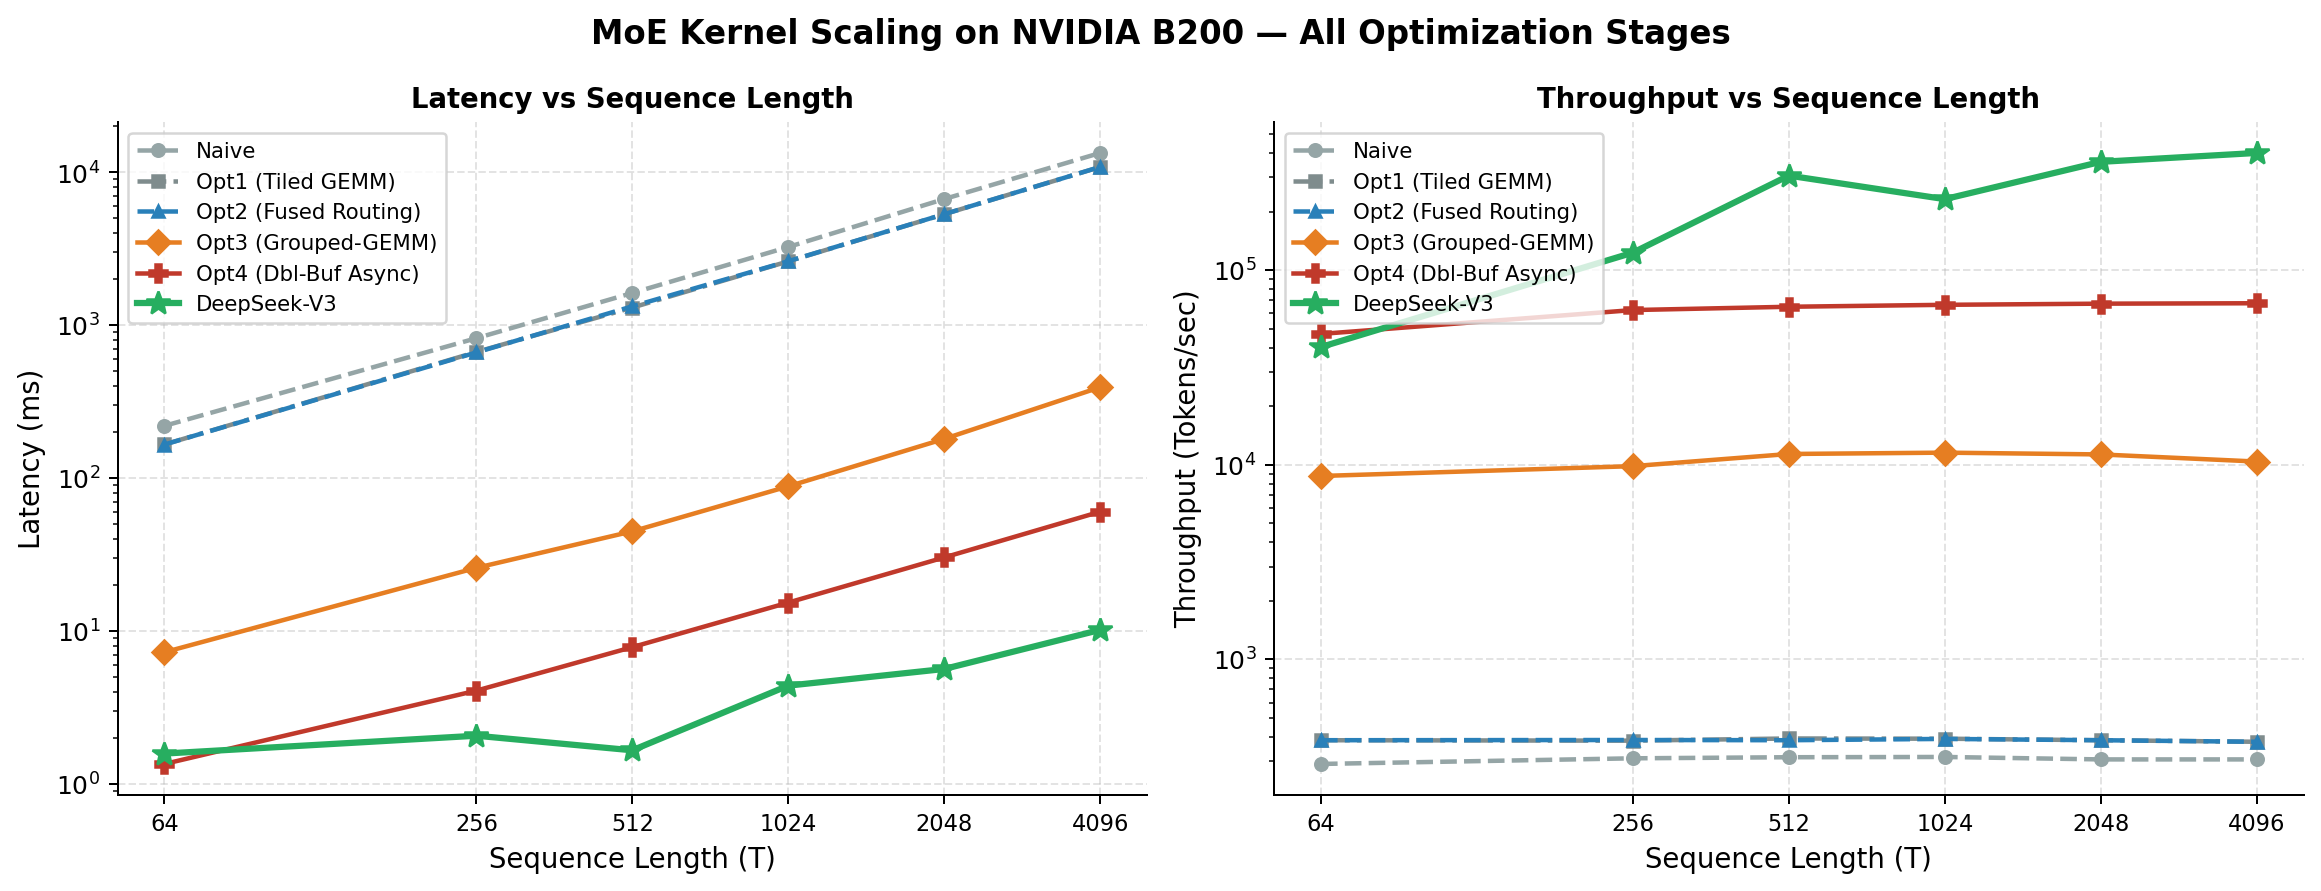
\includegraphics[width=\linewidth]{../figures/moe_scaling_lines.png}
  \caption{MoE kernel latency (left) and throughput (right) across all optimization stages on the NVIDIA B200. Both axes are log-scale. The Grouped-GEMM step (Opt 3) produces the largest single discontinuity; async DMA and DeepSeek routing then push the kernel to the B200 HBM streaming ceiling.}
  \label{fig:scaling}
\end{figure*}

Three phases of improvement are visible in Figure~\ref{fig:scaling}:
\begin{enumerate}
  \item \textbf{Opts 1–2} ($\approx$1.2$\times$): Marginal improvement because the \texttt{gather\_kernel}'s \texttt{block\_size=1} bottleneck was not addressed.
  \item \textbf{Opt 3} ($\approx$30$\times$ over baseline): Grouped-GEMM eliminated both API dispatch overhead and L2 cache thrashing in a single change.
  \item \textbf{Opts 4–DS-V3} ($\approx$200$\times$–1300$\times$): Async DMA and DeepSeek routing together pushed the kernel to the hardware ceiling, with sub-linear scaling at large $T$ indicating effective HBM bandwidth saturation.
\end{enumerate}

% ────────────────────────────────────────────────────────────────────────────
\subsection{Conclusion}
% ────────────────────────────────────────────────────────────────────────────

The optimization journey demonstrates that GPU kernel performance is a moving bottleneck: resolving one constraint consistently exposed the next. The most impactful single change was the Grouped-GEMM refactor (30$\times$ speedup), which required a fundamentally different dispatch model rather than a micro-optimization. The async double-buffering and DeepSeek routing changes then extracted the remaining hardware headroom. Together they deliver a \textbf{1,300$\times$} end-to-end speedup and position the kernel at the B200 HBM streaming ceiling.
